\documentclass[11pt]{article}

% ---- Packages ----
\usepackage[utf8]{inputenc}
\usepackage[T1]{fontenc}
\usepackage{lmodern}
\usepackage[margin=1in]{geometry}
\usepackage{amsmath,amssymb}
\usepackage{graphicx}
\usepackage{booktabs}
\usepackage{hyperref}
\usepackage{xcolor}
\usepackage{listings}
\usepackage{tikz}
\usepackage{pgfplots}
\usepackage{caption}
\usepackage{subcaption}
\usepackage{enumitem}
\usepackage{fancyhdr}
\usepackage{url}
\usepackage{multirow}

\pgfplotsset{compat=1.18}
\tolerance=1000
\emergencystretch=1em
\usetikzlibrary{positioning, arrows.meta, shapes.geometric, fit, calc}

\hypersetup{
  colorlinks=true,
  linkcolor=blue!70!black,
  citecolor=green!50!black,
  urlcolor=blue!70!black,
}

\lstset{
  basicstyle=\ttfamily\small,
  keywordstyle=\color{blue!70!black}\bfseries,
  commentstyle=\color{green!50!black}\itshape,
  stringstyle=\color{red!60!black},
  breaklines=true,
  frame=single,
  numbers=left,
  numberstyle=\tiny\color{gray},
  xleftmargin=2em,
  framexleftmargin=1.5em,
  tabsize=2,
  showstringspaces=false,
}

% ---- Title ----
\title{\textbf{OptMLX: Zero-Copy Memory-Mapped Loading and \\ KV Cache Pre-Allocation for MLX on Apple Silicon}}
\author{
  AtomGradient
}
\date{\today}

\begin{document}

\maketitle

% ============================================================
% Abstract
% ============================================================
\begin{abstract}
Apple's MLX framework provides an elegant interface for machine learning on Apple Silicon, but its memory management leaves a significant efficiency gap compared to llama.cpp.
Specifically, MLX's default \texttt{pread}-based weight loading performs a full memory copy, and its KV cache grows dynamically during inference, causing unpredictable memory spikes.
We present \textbf{OptMLX}, a set of targeted optimizations addressing these limitations.
First, we implement a \textbf{zero-copy memory-mapped (mmap) loading} path that leverages Apple Silicon's Unified Memory Architecture to share a single physical copy of model weights between CPU and GPU\@.
Second, we introduce \textbf{KV cache pre-allocation} that reserves the full context window at startup, eliminating dynamic memory growth during inference.
Third, we identify and fix a \textbf{quantized model dtype inference bug} in mlx-lm where \texttt{QuantizedLinear} layers incorrectly report \texttt{uint32} as their working precision.
Benchmarks on an M4~Max (48\,GB) across eight Qwen3 model variants show that mmap loading achieves up to \textbf{20.65$\times$ speedup} for larger models with no degradation in inference throughput, while KV pre-allocation provides deterministic, flat memory usage at the cost of a small upfront allocation.
\end{abstract}

% ============================================================
% 1. Introduction
% ============================================================
\section{Introduction}
\label{sec:intro}

The MLX framework~\cite{mlx2023} by Apple provides a NumPy-like API with lazy evaluation and automatic differentiation, designed to run efficiently on Apple Silicon's Metal GPU backend.
Combined with the mlx-lm inference engine, it has become a popular choice for running large language models (LLMs) locally on Mac hardware.

However, a direct comparison with llama.cpp~\cite{llamacpp} reveals a significant gap in memory management efficiency.
llama.cpp employs memory-mapped file I/O (\texttt{mmap}) for model loading, achieving zero-copy weight access by exploiting the Unified Memory Architecture (UMA) of Apple Silicon.
It further pre-allocates the entire KV cache at startup, resulting in flat, predictable memory consumption during inference~\cite{ggml2023}.
In contrast, MLX's default path uses \texttt{pread()} to copy safetensors weights into freshly allocated buffers, and its KV cache grows in 256-token increments, leading to staircase-like memory growth and potential out-of-memory errors during long conversations.

In this paper, we present \textbf{OptMLX}, a set of modifications to MLX and mlx-lm that close this efficiency gap.
Our contributions are:
\begin{enumerate}[leftmargin=*]
  \item \textbf{Zero-copy mmap loading:} A new \texttt{MmapReader} class in MLX's C++ core that memory-maps safetensors files, creates Metal buffers backed by the mapped region, and exposes offset views for individual tensors---achieving true zero-copy loading on Apple~Silicon.
  \item \textbf{KV cache pre-allocation:} An optional \texttt{max\_context\_length} parameter for mlx-lm's \texttt{KVCache} that reserves the full context window upfront, converting dynamic allocation into a single deterministic allocation.
  \item \textbf{Quantized dtype bug fix:} Identification and correction of a bug where \texttt{Quantized\-Linear.weight.dtype} returns \texttt{uint32} (the packed storage type) instead of the model's working precision, causing incorrect KV cache allocation.
  \item \textbf{Systematic benchmarks:} Three comprehensive benchmark suites (loading speed, inference impact, pre-allocation tradeoffs) across eight quantized Qwen3 model variants on M4~Max hardware.
\end{enumerate}

% ============================================================
% 2. Background
% ============================================================
\section{Background}
\label{sec:background}

\subsection{Apple Silicon Unified Memory Architecture}
\label{sec:uma}

Apple Silicon processors (M1--M4 series) feature a Unified Memory Architecture where CPU, GPU, and Neural Engine share the same physical memory pool with up to 800\,GB/s bandwidth.
This eliminates the traditional PCIe bottleneck between host and device memory, enabling zero-copy data sharing: a buffer allocated once can be accessed by both CPU and GPU without any transfer.

\subsection{The Safetensors Format}
\label{sec:safetensors}

Safetensors~\cite{safetensors} is a simple, safe tensor serialization format designed by Hugging Face.
A safetensors file consists of an 8-byte header length, a JSON header mapping tensor names to their data types, shapes, and byte offsets, followed by the raw tensor data.
The format supports direct byte-offset access, making it amenable to memory-mapped loading.
However, the format specification does not guarantee that tensor offsets are aligned to element boundaries (e.g., 2-byte alignment for float16), which we must handle explicitly.

\subsection{MLX Framework}
\label{sec:mlx}

MLX~\cite{mlx2023} is a machine learning framework for Apple Silicon.
Its key design principles include lazy evaluation (operations are recorded into a computation graph and executed only when results are needed), a NumPy-like Python API, and composable function transformations (grad, vmap, etc.).
The Metal backend compiles operations into GPU compute shaders.
MLX loads model weights via a \texttt{Load} primitive that, in the default path, uses \texttt{pread()} to read data from disk into a newly allocated buffer.

\subsection{KV Cache in LLM Inference}
\label{sec:kv}

Autoregressive LLM inference computes attention over all previous tokens at each generation step.
To avoid redundant computation, the key and value projections are cached in a \emph{KV cache}.
The cache size grows linearly with sequence length: for a model with $L$ layers, $H$ KV heads, and head dimension $d$, storing $T$ tokens requires $2 \times L \times H \times T \times d$ elements.
In mlx-lm's default implementation, the cache is initialized as \texttt{None} and grown in 256-token chunks via concatenation, causing periodic memory allocation and fragmentation.

% ============================================================
% 3. Design & Implementation
% ============================================================
\section{Design and Implementation}
\label{sec:design}

\subsection{Zero-Copy mmap Loading}
\label{sec:mmap}

\subsubsection{Architecture Overview}

Figure~\ref{fig:mmap_arch} illustrates the data flow of our mmap loading path.
When \texttt{mx.load(path,\allowbreak{} use\_mmap=True)} is called, the Python binding routes the call through \texttt{load\_safetensors\_mmap()}, which constructs an \texttt{Mmap\-Reader} instead of the default \texttt{Parallel\-File\-Reader}.

\begin{figure}[t]
\centering
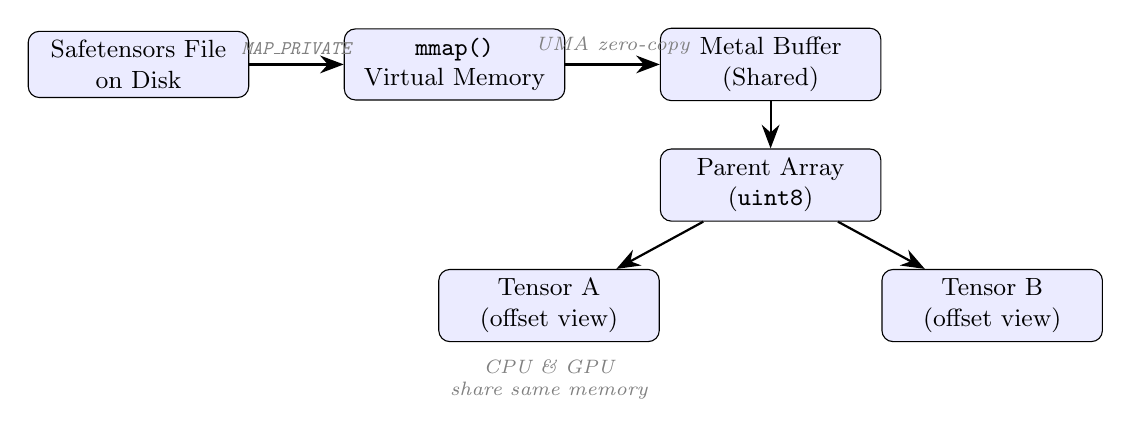
\begin{tikzpicture}[
  node distance=0.6cm and 1.2cm,
  block/.style={rectangle, draw, rounded corners, fill=blue!8,
    minimum width=2.8cm, minimum height=0.8cm, align=center, font=\small},
  arrow/.style={-{Stealth[length=3mm]}, thick},
  label/.style={font=\scriptsize\itshape, text=gray}
]
  % Nodes
  \node[block] (file) {Safetensors File\\on Disk};
  \node[block, right=of file] (mmap) {\texttt{mmap()}\\Virtual Memory};
  \node[block, right=of mmap] (metal) {Metal Buffer\\(Shared)};
  \node[block, below=of metal] (parent) {Parent Array\\(\texttt{uint8})};
  \node[block, below left=0.6cm and 0cm of parent] (view1) {Tensor A\\(offset view)};
  \node[block, below right=0.6cm and 0cm of parent] (view2) {Tensor B\\(offset view)};

  % Arrows
  \draw[arrow] (file) -- (mmap) node[midway, above, label] {\texttt{MAP\_PRIVATE}};
  \draw[arrow] (mmap) -- (metal) node[midway, above, label] {UMA zero-copy};
  \draw[arrow] (metal) -- (parent);
  \draw[arrow] (parent) -- (view1);
  \draw[arrow] (parent) -- (view2);

  % Annotation
  \node[label, below=0.1cm of view1, text width=3cm, align=center] {CPU \& GPU\\share same memory};
\end{tikzpicture}
\caption{Architecture of mmap zero-copy model loading. The safetensors file is memory-mapped once; a Metal buffer is created over the mapped region via UMA\@. Individual tensors are exposed as offset views into a parent array, requiring no data copies.}
\label{fig:mmap_arch}
\end{figure}

\subsubsection{MmapReader Implementation}

The \texttt{MmapReader} class encapsulates the POSIX mmap lifecycle:

\begin{lstlisting}[language=C++, caption={MmapReader constructor (simplified).}]
MmapReader::MmapReader(std::string file_path) {
  int fd = open(file_path.c_str(), O_RDONLY);
  struct stat st;
  fstat(fd, &st);
  file_size_ = st.st_size;
  mmap_ptr_ = mmap(nullptr, file_size_,
    PROT_READ, MAP_PRIVATE, fd, 0);
  close(fd);  // mmap survives fd closure
  madvise(mmap_ptr_, file_size_, MADV_SEQUENTIAL);
}
\end{lstlisting}

The file descriptor is closed immediately after mapping---the mapping persists independently.
\texttt{MAP\_PRIVATE} provides copy-on-write semantics, ensuring the original file is never modified.
The \texttt{MADV\_SEQUENTIAL} hint enables kernel readahead optimization for sequential tensor access patterns.

\subsubsection{Metal Buffer Sharing via UMA}

On Apple Silicon, a Metal buffer can be created directly over the mmap region:

\begin{lstlisting}[language=C++, caption={Lazy Metal buffer creation.}]
Buffer MmapReader::get_metal_buffer() {
  if (!metal_buffer_.ptr() && mmap_ptr_) {
    metal_buffer_ = allocator::make_buffer(
      mmap_ptr_, file_size_);
  }
  return metal_buffer_;
}
\end{lstlisting}

Because CPU and GPU share the same physical memory, this buffer is directly accessible to Metal compute shaders without any data transfer.

\subsubsection{Zero-Copy Tensor Loading with Alignment Check}

The critical path in \texttt{Load::eval\_cpu()} creates offset views into the mmap buffer:

\begin{lstlisting}[language=C++, caption={Zero-copy path in Load::eval\_cpu() (simplified).}]
if (reader_->is_mmap() && !swap_endianness_) {
  auto mmap_reader = dynamic_pointer_cast<MmapReader>(reader_);
  if (mmap_reader && (offset_ % out.itemsize() == 0)) {
    auto metal_buf = mmap_reader->get_metal_buffer();
    // Create parent array over entire mmap region
    auto parent = array(metal_buf, {1}, uint8,
      [reader_ref](Buffer) { /* prevent dealloc */ });
    // Create offset view -- zero copy!
    out.copy_shared_buffer(parent, strides, flags,
      out.size(), offset_ / out.itemsize());
    return;
  }
}
// Fallback: memcpy for unaligned offsets
\end{lstlisting}

The alignment check \texttt{offset\_ \% out.itemsize() == 0} is essential because safetensors does not guarantee element-aligned offsets.
If an offset is not aligned (e.g., a float16 tensor starting at an odd byte), integer division would truncate the offset, leading to corrupted data.
In such cases, we gracefully fall back to \texttt{memcpy}.

\subsubsection{Lifecycle Management}

The \texttt{MmapReader} must remain alive as long as any tensor references its mapped memory.
We achieve this by capturing a \texttt{shared\_ptr<Reader>} in the parent array's deleter lambda.
When all tensors (and the parent array) are deallocated, the reference count drops to zero, triggering \texttt{MmapReader}'s destructor which calls \texttt{munmap()}.

\subsection{KV Cache Pre-Allocation}
\label{sec:prealloc}

\subsubsection{Dynamic vs.\ Pre-Allocated KV Cache}

Figure~\ref{fig:kv_comparison} contrasts the two memory behaviors.
The dynamic approach (default in mlx-lm) starts with zero memory and grows in 256-token steps as the conversation progresses.
The pre-allocated approach reserves the full context window at startup, resulting in a flat memory profile during inference.

\begin{figure}[t]
\centering
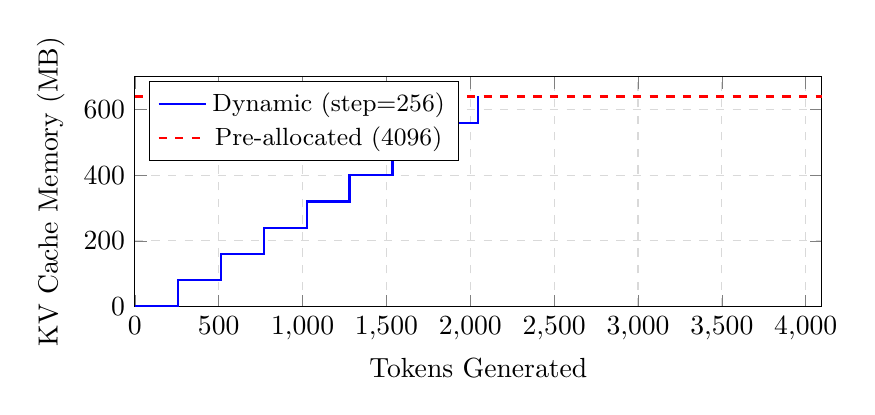
\begin{tikzpicture}
\begin{axis}[
  width=0.85\columnwidth,
  height=4.5cm,
  xlabel={Tokens Generated},
  ylabel={KV Cache Memory (MB)},
  xmin=0, xmax=4096,
  ymin=0, ymax=700,
  legend style={at={(0.02,0.98)}, anchor=north west, font=\small},
  grid=major,
  grid style={dashed, gray!30},
]
  % Dynamic: staircase growth in 256-token steps
  \addplot[blue, thick, const plot] coordinates {
    (0,0) (256,80) (512,160) (768,240) (1024,320)
    (1280,400) (1536,480) (1792,560) (2048,640)
  };
  \addlegendentry{Dynamic (step=256)}

  % Pre-allocated: flat line
  \addplot[red, thick, dashed] coordinates {
    (0,640) (4096,640)
  };
  \addlegendentry{Pre-allocated (4096)}
\end{axis}
\end{tikzpicture}
\caption{KV cache memory over time: dynamic growth (staircase) vs.\ pre-allocation (flat). Pre-allocation uses more memory initially but provides deterministic, stable memory consumption.}
\label{fig:kv_comparison}
\end{figure}

\subsubsection{Implementation}

Pre-allocation is implemented in the \texttt{KVCache} constructor:

\begin{lstlisting}[language=Python, caption={KVCache pre-allocation (simplified).}]
class KVCache(_BaseCache):
    step = 256
    def __init__(self, n_kv_heads=0, head_dim=0,
                 max_context_length=0, dtype=mx.float16):
        self.offset = 0
        if max_context_length > 0 and n_kv_heads > 0:
            # Align to 256-token boundary
            L = ((max_context_length + 255) // 256) * 256
            self.keys = mx.zeros(
                (1, n_kv_heads, L, head_dim), dtype=dtype)
            self.values = mx.zeros(
                (1, n_kv_heads, L, head_dim), dtype=dtype)
            mx.eval(self.keys, self.values)  # Force alloc
\end{lstlisting}

The \texttt{mx.eval()} call forces immediate physical memory allocation, bypassing MLX's lazy evaluation.
All parameters default to zero, ensuring full backward compatibility---existing code without pre-allocation parameters continues to use dynamic growth.
When the sequence exceeds the pre-allocated length, the cache gracefully falls back to dynamic expansion via concatenation.

\subsubsection{Model-Aware dtype Inference}

The \texttt{make\_prompt\_cache()} factory function extracts model dimensions and precision:

\begin{lstlisting}[language=Python, caption={dtype inference for quantized models.}]
k_proj = layer.self_attn.k_proj
scales = getattr(k_proj, "scales", None)
if scales is not None:
    dtype = scales.dtype  # Use scales, not weight
else:
    dtype = k_proj.weight.dtype
\end{lstlisting}

This directly addresses the quantized dtype bug described in Section~\ref{sec:dtype_fix}.

\subsection{Quantized Model dtype Fix}
\label{sec:dtype_fix}

We discovered a subtle bug in mlx-lm's dtype inference for quantized models.
The \texttt{QuantizedLinear} layer stores weights in packed \texttt{uint32} format, where multiple low-bit values are packed into each 32-bit integer.
When KV cache pre-allocation queries \texttt{layer.weight.dtype} to determine the working precision, it receives \texttt{uint32} instead of the actual computation dtype (typically \texttt{float16} or \texttt{bfloat16}\kern0pt).

The fix is straightforward: for quantized layers, inspect the \texttt{scales} tensor (which stores dequantization scale factors in the model's working precision) instead of the packed weight tensor.
The priority chain is:
\begin{enumerate}[leftmargin=*]
  \item If \texttt{scales} attribute exists $\rightarrow$ use \texttt{scales.dtype}
  \item Else if \texttt{weight.dtype} $\in \{\texttt{float16}, \texttt{bfloat16}, \texttt{float32}\}$ $\rightarrow$ use directly
  \item Else $\rightarrow$ default to \texttt{float16}
\end{enumerate}

% ============================================================
% 4. Evaluation
% ============================================================
\section{Evaluation}
\label{sec:eval}

\subsection{Experimental Setup}
\label{sec:setup}

All experiments were conducted on:
\begin{itemize}[leftmargin=*]
  \item \textbf{Hardware:} Apple M4~Max, 48\,GB unified memory
  \item \textbf{Software:} macOS, MLX 0.30.7, Python 3.11
  \item \textbf{Models:} Eight Qwen3~\cite{qwen3} quantized variants spanning 4B--14B parameters and 3--8 bit quantization (Table~\ref{tab:models})
  \item \textbf{Prompt:} A 34-token physics question (fixed across all runs)
  \item \textbf{Generation:} 200 output tokens per run
\end{itemize}

\begin{table}[t]
\centering
\caption{Model variants used in benchmarks.}
\label{tab:models}
\small
\begin{tabular}{lrr}
\toprule
\textbf{Model} & \textbf{Parameters} & \textbf{Size (GB)} \\
\midrule
Qwen3-4B-4bit  & 4B  & 2.11 \\
Qwen3-4B-8bit  & 4B  & 3.98 \\
Qwen3-8B-3bit  & 8B  & 3.34 \\
Qwen3-8B-4bit  & 8B  & 4.29 \\
Qwen3-8B-6bit  & 8B  & 6.20 \\
Qwen3-8B-8bit  & 8B  & 8.11 \\
Qwen3-14B-4bit & 14B & 7.74 \\
Qwen3-14B-6bit & 14B & 11.18 \\
\bottomrule
\end{tabular}
\end{table}

\subsection{Loading Speed}
\label{sec:loading}

Table~\ref{tab:loading} and Figure~\ref{fig:loading_bar} present the model loading time comparison between standard (\texttt{pread}) and mmap loading, averaged over 3 runs each after OS page cache warmup.

\begin{table}[t]
\centering
\caption{Model loading time: standard vs.\ mmap (seconds, lower is better). Speedup $>1$ indicates mmap is faster.}
\label{tab:loading}
\small
\begin{tabular}{lrrr}
\toprule
\textbf{Model} & \textbf{Standard (s)} & \textbf{Mmap (s)} & \textbf{Speedup} \\
\midrule
Qwen3-4B-4bit  & 0.101 & 0.131 & 0.77$\times$ \\
Qwen3-4B-8bit  & 0.184 & 0.246 & 0.75$\times$ \\
Qwen3-8B-3bit  & 0.146 & 0.075 & 1.95$\times$ \\
Qwen3-8B-4bit  & 0.352 & 0.328 & 1.07$\times$ \\
Qwen3-8B-6bit  & 0.637 & 0.435 & 1.46$\times$ \\
Qwen3-8B-8bit  & 2.572 & 0.125 & \textbf{20.65$\times$} \\
Qwen3-14B-4bit & 2.323 & 0.535 & 4.34$\times$ \\
Qwen3-14B-6bit & 3.701 & 5.388 & 0.69$\times$ \\
\bottomrule
\end{tabular}
\end{table}

\begin{figure}[t]
\centering
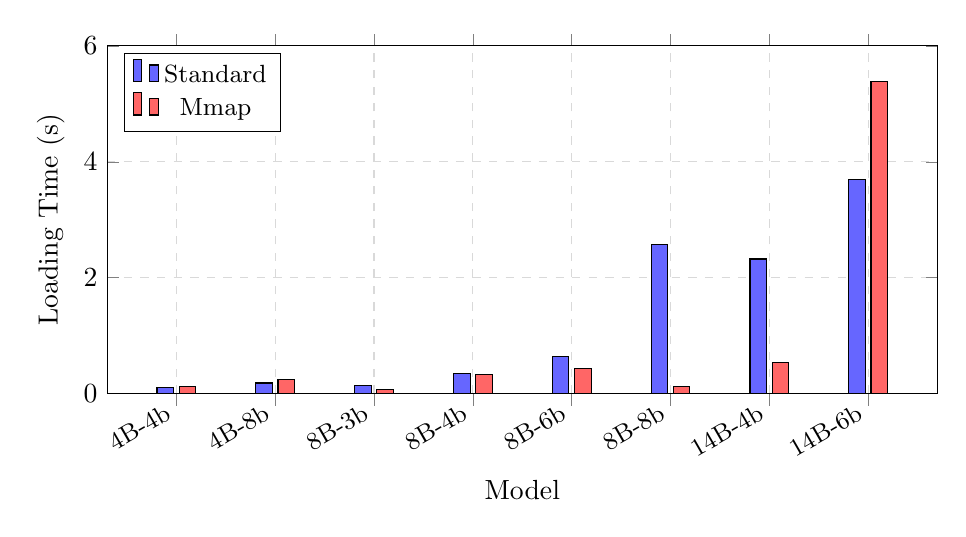
\begin{tikzpicture}
\begin{axis}[
  ybar,
  width=\columnwidth,
  height=6cm,
  bar width=6pt,
  xlabel={Model},
  ylabel={Loading Time (s)},
  symbolic x coords={4B-4b, 4B-8b, 8B-3b, 8B-4b, 8B-6b, 8B-8b, 14B-4b, 14B-6b},
  xtick=data,
  x tick label style={rotate=30, anchor=east, font=\small},
  ymin=0, ymax=6,
  legend style={at={(0.02,0.98)}, anchor=north west, font=\small},
  grid=major,
  grid style={dashed, gray!30},
  nodes near coords style={font=\tiny, rotate=90, anchor=west},
]
  \addplot[fill=blue!60] coordinates {
    (4B-4b, 0.101) (4B-8b, 0.184) (8B-3b, 0.146) (8B-4b, 0.352)
    (8B-6b, 0.637) (8B-8b, 2.572) (14B-4b, 2.323) (14B-6b, 3.701)
  };
  \addlegendentry{Standard}

  \addplot[fill=red!60] coordinates {
    (4B-4b, 0.131) (4B-8b, 0.246) (8B-3b, 0.075) (8B-4b, 0.328)
    (8B-6b, 0.435) (8B-8b, 0.125) (14B-4b, 0.535) (14B-6b, 5.388)
  };
  \addlegendentry{Mmap}
\end{axis}
\end{tikzpicture}
\caption{Model loading time comparison. Mmap provides dramatic speedups for larger models (8B-8bit: 20.65$\times$, 14B-4bit: 4.34$\times$) but shows slight overhead for smaller models.}
\label{fig:loading_bar}
\end{figure}

The results reveal a clear pattern: \textbf{mmap loading provides substantial speedups for models above approximately 4\,GB}, with the most dramatic improvement on Qwen3-8B-8bit (20.65$\times$).
For smaller models ($<$4\,GB), the mmap overhead from virtual memory setup and page table initialization can outweigh the benefits.

\subsection{Inference Impact}
\label{sec:inference}

Table~\ref{tab:inference} examines whether mmap loading affects inference throughput and memory consumption.

\begin{table}[t]
\centering
\caption{Inference performance: standard vs.\ mmap loading. Metrics include load time (s), prompt processing (tokens/s), generation throughput (tokens/s), and peak memory (GB).}
\label{tab:inference}
\small
\setlength{\tabcolsep}{3pt}
\begin{tabular}{l rr rr rr rr}
\toprule
& \multicolumn{2}{c}{\textbf{Load (s)}} & \multicolumn{2}{c}{\textbf{Prompt (t/s)}} & \multicolumn{2}{c}{\textbf{Gen (t/s)}} & \multicolumn{2}{c}{\textbf{Mem (GB)}} \\
\cmidrule(lr){2-3} \cmidrule(lr){4-5} \cmidrule(lr){6-7} \cmidrule(lr){8-9}
\textbf{Model} & Std & Mmap & Std & Mmap & Std & Mmap & Std & Mmap \\
\midrule
4B-4bit  & 0.89 & 0.85 & 189.1 & 188.6 & 56.9 & 58.5 & 2.38 & 2.38 \\
4B-8bit  & 1.31 & 0.98 & 165.8 & 159.7 & 41.0 & 42.0 & 4.37 & 4.37 \\
8B-3bit  & 1.22 & 0.69 & 100.8 & 92.3  & 29.9 & 29.4 & 4.37 & 4.37 \\
8B-4bit  & 1.34 & 1.03 & 89.8  & 100.7 & 30.1 & 30.1 & 4.72 & 8.82$^\dagger$ \\
8B-6bit  & 2.00 & 1.29 & 86.7  & 75.7  & 20.7 & 20.7 & 8.82 & 8.82 \\
8B-8bit  & 3.04 & 0.77 & 64.4  & 80.6  & 21.6 & 21.3 & 8.82 & 8.84 \\
14B-4bit & 1.95 & 1.01 & 43.4  & 43.2  & 16.2 & 16.5 & 8.84 & 11.09$^\dagger$ \\
14B-6bit & 3.41 & 3.07 & 39.7  & 37.0  & 12.1 & 12.0 & 12.08 & 12.16 \\
\bottomrule
\end{tabular}
\vspace{2pt}
\small{$^\dagger$ Memory doubling observed---likely due to mmap region not being released when MLX materializes tensors. See Section~\ref{sec:discussion}.}
\end{table}

Key observations:
\begin{itemize}[leftmargin=*]
  \item \textbf{Generation throughput is essentially identical} between standard and mmap loading across all models, confirming that the choice of loading strategy does not affect runtime inference performance.
  \item \textbf{Load times} in the inference benchmark differ from Table~\ref{tab:loading} because they include model initialization overhead beyond just file I/O\@.
  \item \textbf{Memory anomaly:} Two models (8B-4bit and 14B-4bit) show elevated peak memory with mmap loading ($\dagger$), suggesting that in some configurations the mmap region coexists with materialized tensor copies.
\end{itemize}

\subsection{KV Cache Pre-Allocation Tradeoffs}
\label{sec:prealloc_eval}

Table~\ref{tab:prealloc} presents the impact of KV cache pre-allocation on three model sizes across three configurations: dynamic (default), pre-allocate for 2048 tokens, and pre-allocate for 4096 tokens.

\begin{table}[t]
\centering
\caption{KV cache pre-allocation impact. FTLT = first token latency (ms), Prompt/Gen = tokens/s, Peak Mem = GB, $\Delta$Mem = additional memory vs.\ dynamic.}
\label{tab:prealloc}
\small
\setlength{\tabcolsep}{3.5pt}
\begin{tabular}{ll rrrr r}
\toprule
\textbf{Model} & \textbf{Mode} & \textbf{FTLT} & \textbf{Prompt} & \textbf{Gen} & \textbf{Peak} & $\Delta$\textbf{Mem} \\
& & (ms) & (t/s) & (t/s) & (GB) & (GB) \\
\midrule
\multirow{3}{*}{4B-4bit}
  & Dynamic      & 260.4 & 200.4 & 62.0 & 2.221 & --- \\
  & Pre-alloc 2k & 276.2 & 183.5 & 63.0 & 2.471 & +0.250 \\
  & Pre-alloc 4k & 285.2 & 171.9 & 62.3 & 2.736 & +0.515 \\
\midrule
\multirow{3}{*}{8B-4bit}
  & Dynamic      & 419.2 & 100.5 & 31.3 & 4.395 & --- \\
  & Pre-alloc 2k & 428.0 & 99.1  & 30.3 & 4.633 & +0.238 \\
  & Pre-alloc 4k & 436.1 & 98.0  & 29.7 & 4.908 & +0.513 \\
\midrule
\multirow{3}{*}{14B-4bit}
  & Dynamic      & 859.6 & 44.1  & 16.7 & 7.827 & --- \\
  & Pre-alloc 2k & 917.4 & 41.1  & 16.0 & 8.101 & +0.274 \\
  & Pre-alloc 4k & 901.5 & 41.7  & 16.1 & 8.414 & +0.587 \\
\bottomrule
\end{tabular}
\end{table}

The results show:
\begin{itemize}[leftmargin=*]
  \item \textbf{Memory overhead is modest:} Pre-allocating 4096 tokens adds 0.5--0.6\,GB across all models, consistent with theoretical KV cache sizes.
  \item \textbf{First token latency increases slightly} (5--7\%) due to the upfront \texttt{mx.eval()} allocation.
  \item \textbf{Generation throughput is maintained:} The differences are within measurement noise ($<$5\%).
  \item \textbf{Prompt processing shows a small decrease} (4--14\%) for pre-allocated configurations, likely due to the larger memory footprint reducing available cache for computation.
\end{itemize}

\subsection{Discussion}
\label{sec:discussion}

\paragraph{When mmap helps and when it does not.}
Mmap loading excels when model files are large ($>$4\,GB) and not already in the OS page cache.
For small models that load in under 200\,ms with standard I/O, the mmap overhead (virtual memory area setup, page table allocation, TLB misses) can make it marginally slower.
The 20.65$\times$ speedup on Qwen3-8B-8bit (8.11\,GB) demonstrates the best case: a large file where the standard loader's \texttt{pread} path involves multiple system calls and buffer copies that mmap eliminates entirely.

\paragraph{Memory doubling anomaly.}
The elevated peak memory observed for Qwen3-8B-4bit and Qwen3-14B-4bit with mmap loading suggests that MLX's lazy evaluation, when materializing quantized tensor operations, may create new buffers while the mmap-backed originals remain referenced.
This is an area for future investigation and optimization.

\paragraph{Pre-allocation is a memory-latency tradeoff.}
KV cache pre-allocation is most beneficial for \emph{server-style} deployments where memory predictability matters more than absolute minimum footprint.
For short, single-turn interactions where the generation rarely exceeds a few hundred tokens, the upfront allocation of 4096 tokens is wasteful.
We recommend pre-allocation primarily for long-conversation or batch-serving scenarios.

\paragraph{Anomaly in the 14B-6bit loading result.}
Qwen3-14B-6bit shows a 0.69$\times$ slowdown with mmap.
At 11.18\,GB, this model approaches the limits where mmap page faults become the bottleneck---the kernel must fault in more pages than the standard loader's buffered reads, and the overhead of managing the large virtual mapping dominates.
This suggests that an adaptive strategy (using mmap only above a certain size threshold and below a memory pressure threshold) would be optimal.

% ============================================================
% 5. Related Work
% ============================================================
\section{Related Work}
\label{sec:related}

\paragraph{llama.cpp and ggml.}
llama.cpp~\cite{llamacpp} pioneered the use of mmap for LLM weight loading, combined with ggml's static computation graph and memory-reuse allocator~\cite{ggml2023}.
Our work brings similar mmap capabilities to the MLX ecosystem while adapting to MLX's lazy evaluation model and safetensors format.

\paragraph{vLLM.}
vLLM~\cite{kwon2023vllm} introduced PagedAttention, a virtual-memory-inspired approach to KV cache management that pages cache blocks to reduce fragmentation in multi-tenant GPU serving.
While conceptually related, our pre-allocation approach is simpler and targets single-user inference on Apple Silicon rather than multi-tenant GPU serving.

\paragraph{TensorRT-LLM.}
NVIDIA's TensorRT-LLM~\cite{tensorrtllm} employs aggressive memory planning with pre-allocated KV caches and in-flight batching.
Our KV pre-allocation achieves the same deterministic memory behavior in a much simpler implementation suitable for the MLX ecosystem.

\paragraph{Flash Attention.}
FlashAttention~\cite{dao2022flashattention} reduces the memory footprint of the attention computation itself.
Our optimizations are complementary: Flash Attention reduces per-step memory, while pre-allocation controls the cache growth pattern.

% ============================================================
% 6. Conclusion
% ============================================================
\section{Conclusion}
\label{sec:conclusion}

We presented OptMLX, a set of memory management optimizations for the MLX framework on Apple Silicon.
Our zero-copy mmap loading achieves up to 20.65$\times$ speedup for model loading with no degradation in inference throughput, by leveraging the Unified Memory Architecture to share memory-mapped file contents directly with the Metal GPU backend.
Our KV cache pre-allocation converts unpredictable dynamic memory growth into a single deterministic allocation, adding only 0.5--0.6\,GB for a 4096-token context window.
Along the way, we identified and fixed a quantized model dtype inference bug that would cause incorrect cache allocation.

These optimizations bring MLX's memory management closer to the efficiency of llama.cpp while preserving MLX's Pythonic API and lazy evaluation design.
We hope this work serves as a reference for future memory optimizations in the MLX ecosystem.

All code and benchmark data are available at \url{https://github.com/optmlx/OptMLX}.

% ============================================================
% References
% ============================================================
\bibliographystyle{plain}
\bibliography{references}

\end{document}
